\documentclass{scrartcl}
\usepackage[utf8]{inputenc}
\usepackage{hyperref}
\usepackage{url}
\usepackage{natbib}
\usepackage{graphicx}
\usepackage{cleveref} % this must be the last package to be loaded
\usepackage{bookmark}

\newcommand{\emailaddr}[1]{\href{mailto:#1}{\texttt{#1}}}

\title{\LARGE
    Liar's Poker 
}

\author{
    Francesco Buda \\ \emailaddr{francesco.buda3@studio.unibo.it}
    \and
    Emanuele Sanchi \\ \emailaddr{emanuele.sanchi@studio.unibo.it}
    \and
    Tommaso Severi \\ \emailaddr{tommaso.severi2@studio.unibo.it}
}

\date{Febraury 2025}

\begin{document}

\maketitle

\begin{abstract}
    Up to $\sim$2000 characters briefly describing the project.
\end{abstract}

% \section*{Disclaimer (if needed)}

% During the preparation of this work, the author(s) used [NAME TOOL / SERVICE] to [REASON].

% After using this tool/service, 
% the author(s) reviewed and edited the content as needed 
% and take(s) full responsibility for the content of the final report/artifact.

% \section*{Quick \LaTeX{} suggestions}

% If you need to cite a reference, you can use the \texttt{cite} command, 
% like providing the BibTex key of some entry in the \texttt{references.bib} file, 
% e.g.: \cite{adams1995hitchhiker}.

% You can find pre-coocked BibTex entries for most Computer Science papers on \href{https://dblp.uni-trier.de/}{DBLP}.

% If you need to include an image,
% let \LaTeX{} decide where to put it by using the \texttt{figure} environment,
% with a \texttt{includegraphics} command inside it.
% %
% If your need to reference a figure,
% use the \texttt{label} command to assign a label to the figure,
% and then use the \texttt{cref} command to reference it.
% %
% Put figures in the \texttt{figures} folder.
% %
% A complete example is shown in \cref{fig:universe}.

% \begin{figure}
%     \centering
%     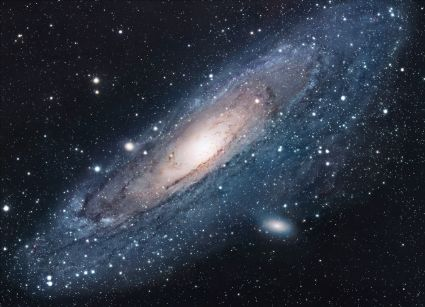
\includegraphics[width=0.5\textwidth]{figures/universe.jpg}
%     \caption{This is an example image}
%     \label{fig:universe}
% \end{figure}

% Do not put any placement constraint on figures,
% such as \texttt{[h]} or \texttt{[h!]}.
% %
% Same considerations apply for other floating elements 
% (e.g. tables, algorithms, listings, etc.).

% Do not use the \texttt{\textbackslash\textbackslash} or \texttt{\textbackslash newline} commands to break lines.

% Just leave an empty line between two paragraphs to start a new one.
% %
% The new line will be automatically indented.
% %
% This is intended: it is the \LaTeX{} way to separate capoverses.

\section{Concept}\label{concept}

Here you should explain:

\begin{itemize}
  \item The type of product developed with that project, for example
  (non-exhaustive):

  \begin{itemize}
    \item Application (with GUI, be it mobile, web, or desktop)
    \item Command-line application (CLI could be used by humans or scripts)
    \item Library
    \item Web-service(s)
  \end{itemize}
  \item Use case collection

  \begin{itemize}
    \item \emph{where} are the users?
    \item \emph{when} and \emph{how frequently} do they interact with the
    system?
    \item \emph{how} do they \emph{interact} with the system? which
    \emph{devices} are they using?
    \item does the system need to \emph{store} user's \textbf{data}?
    \emph{which}? \emph{where}?
    \item most likely, there will be \emph{multiple} \textbf{roles}
  \end{itemize}
\end{itemize}

\section{Requirements}\label{requirements}

\begin{itemize}
  \item The requirements must explain \textbf{what} (not how) the software
  being produced should do.

  \begin{itemize}
    \item you should not focus on the particular problems, but exclusively on
    what you want the application to do.
  \end{itemize}
  \item Requirements must be clearly identified, and possibly numbered
  \item Requirements are divided into:

  \begin{itemize}
    \item \textbf{Functional}: some functionality the software should provide
    to the user
    \item \textbf{Non-functional}: requirements that do not directly concern
    behavioural aspects, such as consistency, availability, etc.
    \item \textbf{Implementation}: constrain the entire phase of system
    realization, for instance by requiring the use of a specific
    programming language and/or a specific software tool

    \begin{itemize}
      \item these constraints should be adequately justified by political /
      economic / administrative reasons\ldots{}
      \item \ldots{} otherwise, implementation choices should emerge \emph{as
      a consequence of} design
    \end{itemize}
  \end{itemize}
  \item If there are domain-specific terms, these should be explained in a
  glossary
  \item Each requirement must have its own \textbf{acceptance criteria}

  \begin{itemize}
    \item these will be important for the validation phase
  \end{itemize}
\end{itemize}

\section{Design}\label{design}

This chapter explains the strategies used to meet the requirements
identified in the analysis. Ideally, the design should be the same,
regardless of the technological choices made during the implementation
phase.

\begin{quote}
You can re-order the sections as you prefer, but all the sections must
be present in the end
\end{quote}

\subsection{Architecture}\label{architecture}

  The architecture of the system is a classic MVC where:
  \begin{itemize}
    \item Model are the classes that represents players and cards
    \item View is UI realized with Web components
    \item Controller is the class that manages the game logic
  \end{itemize}
  For the communication architecture and the distributed part, we opted for a client-server architecture using also a publish-subscribe pattern. \newline
  The idea is that the broker manages the communication between the clients and the server, and the server manages the game logic.\newline
  The server is the one that creates the game; then the clients can join the game publishing their nickname to the broker; every time a new player joins the game, it automatically subscribe to the game topics.\newline
  All the clients are subscribed to the same topic, so they can receive the messages from the server (eg. moves, game status, etc.).\newline

  We choose this architecture because it is simple and it is suitable for our project. In fact, using a publish-subscribe architecture, clients have not to request the server for the game status, but they receive it automatically when the server publishes it (and so on for the other messages).

\subsection{Infrastructure}\label{infrastructure}

  \begin{itemize}
    \item both players and server are components of the pub-sub model
    \item there is one server that manages the game logic so is the only one who can publish messages on some specific topics
    \item there is a broker that manages the communication between the clients and the server
    \item data aren't store permanently, so there is no need for a database 
    \item there aren't authentication mechanisms so every one who knows the broker address can join the game

  \end{itemize}
  Components are distributed over all the network, so they can be on different machines and different networks. For semplicity, we used the same network for all the components and the same machine for server and broker. \newline
  To find each other, the components use the broker address and the topics to which they have to subscribe or publish; so clients are only required to know the broker address to join the game. \newline
  Components are named using a nickname (unique) that every body choose when they join the game.


\begin{figure}[h]
  \caption{Architecture diagram}
  \centering
  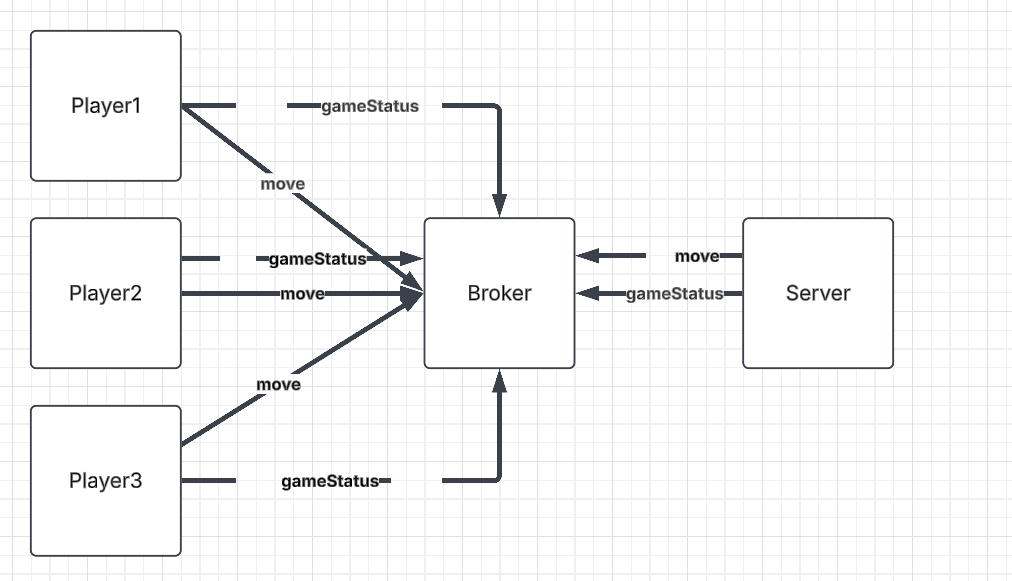
\includegraphics[scale=0.5]{figures/pubsubdiagram.png}
  \end{figure}

  Dotted lines are for subscribe messages, while solid lines are for publish messages. \newline

\subsection{Modelling}\label{modelling}

\begin{itemize}
  \item which \textbf{domain entities} are there?

  \begin{itemize}
    \item e.g.~\emph{users}, \emph{products}, \emph{orders}, \emph{etc.}
  \end{itemize}
  \item how do \emph{domain entities} \textbf{map to} \emph{infrastructural
  components}?

  \begin{itemize}
    \item e.g.~state of a video game on central server, while
    inputs/representations on clients
    \item e.g.~where to store messages in an IM app? for how long?
  \end{itemize}
  \item which \textbf{domain events} are there?

  \begin{itemize}
    \item e.g.~\emph{user registered}, \emph{product added to cart},
    \emph{order placed}, \emph{etc.}
  \end{itemize}
  \item which sorts of \textbf{messages} are exchanged?

  \begin{itemize}
    \item e.g.~\emph{commands}, \emph{events}, \emph{queries}, \emph{etc.}
  \end{itemize}
  \item what information does the \textbf{state} of the system comprehend

  \begin{itemize}
    \item e.g.~\emph{users' data}, \emph{products' data}, \emph{orders' data},
    \emph{etc.}
  \end{itemize}
\end{itemize}

\begin{quote}
Class diagram are welcome here
\end{quote}

\subsection{Interaction}\label{interaction}

\begin{itemize}
  \item how do components \emph{communicate}? \emph{when}? \emph{what}?
  \item \emph{which} \textbf{interaction patterns} do they enact?
\end{itemize}

\begin{quote}
Sequence diagrams are welcome here
\end{quote}

\subsection{Behaviour}\label{behaviour}

\begin{itemize}
  \item how does \emph{each} component \textbf{behave} individually (e.g.~in
  \emph{response} to \emph{events} or messages)?

  \begin{itemize}
    \item some components may be \emph{stateful}, others \emph{stateless}
  \end{itemize}
  \item which components are in charge of updating the \textbf{state} of the
  system? \emph{when}? \emph{how}?
\end{itemize}

\begin{quote}
State diagrams are welcome here
\end{quote}

\subsection{Data and Consistency
Issues}\label{data-and-consistency-issues}

\begin{itemize}
  \item Is there any data that needs to be stored?

  \begin{itemize}
    \item \emph{what} data? \emph{where}? \emph{why}?
  \end{itemize}
  \item how should \emph{persistent data} be \textbf{stored}?

  \begin{itemize}
    \item e.g.~relations, documents, key-value, graph, etc.
    \item why?
  \end{itemize}
  \item Which components perform queries on the database?

  \begin{itemize}
    \item \emph{when}? \emph{which} queries? \emph{why}?
    \item concurrent read? concurrent write? why?
  \end{itemize}
  \item Is there any data that needs to be shared between components?

  \begin{itemize}
    \item \emph{why}? \emph{what} data?
  \end{itemize}
\end{itemize}

\subsection{Fault-Tolerance}\label{fault-tolerance}

\begin{itemize}
  \item Is there any form of data \textbf{replication} / federation / sharing?

  \begin{itemize}
    \item \emph{why}? \emph{how} does it work?
  \end{itemize}
  \item Is there any \textbf{heart-beating}, \textbf{timeout}, \textbf{retry
  mechanism}?

  \begin{itemize}
    \item \emph{why}? \emph{among} which components? \emph{how} does it work?
  \end{itemize}
  \item Is there any form of \textbf{error handling}?

  \begin{itemize}
    \item \emph{what} happens when a component fails? \emph{why}? \emph{how}?
  \end{itemize}
\end{itemize}

\subsection{Availability}\label{availability}

\begin{itemize}
  \item Is there any \textbf{caching} mechanism?

  \begin{itemize}
    \item \emph{where}? \emph{why}?
  \end{itemize}
  \item Is there any form of \textbf{load balancing}?

  \begin{itemize}
    \item \emph{where}? \emph{why}?
  \end{itemize}
  \item In case of \textbf{network partitioning}, how does the system behave?

  \begin{itemize}
    \item \emph{why}? \emph{how}?
  \end{itemize}
\end{itemize}

\subsection{Security}\label{security}

\begin{itemize}
  \item Is there any form of \textbf{authentication}?

  \begin{itemize}
    \item \emph{where}? \emph{why}?
  \end{itemize}
  \item Is there any form of \textbf{authorization}?

  \begin{itemize}
    \item which sort of \emph{access control}?
    \item which sorts of users / \emph{roles}? which \emph{access rights}?
  \end{itemize}
  \item Are \textbf{cryptographic schemas} being used?

  \begin{itemize}
    \item e.g.~token verification,
    \item e.g.~data encryption, etc.
  \end{itemize}
\end{itemize}

\begin{center}\rule{0.5\linewidth}{0.5pt}\end{center}

\section{Implementation}\label{implementation}

\begin{itemize}
  \item which \textbf{network protocols} to use?

  \begin{itemize}
    \item e.g.~UDP, TCP, HTTP, WebSockets, gRPC, XMPP, AMQP, MQTT, etc.
  \end{itemize}
  \item how should \emph{in-transit data} be \textbf{represented}?

  \begin{itemize}
    \item e.g.~JSON, XML, YAML, Protocol Buffers, etc.
  \end{itemize}
  \item how should \emph{databases} be \textbf{queried}?

  \begin{itemize}
    \item e.g.~SQL, NoSQL, etc.
  \end{itemize}
  \item how should components be \emph{authenticated}?

  \begin{itemize}
    \item e.g.~OAuth, JWT, etc.
  \end{itemize}
  \item how should components be \emph{authorized}?

  \begin{itemize}
    \item e.g.~RBAC, ABAC, etc.
  \end{itemize}
\end{itemize}

\subsection{Technological details}\label{technological-details}

\begin{itemize}
  \item any particular \emph{framework} / \emph{technology} being exploited
  goes here
\end{itemize}

\section{Validation}\label{validation}

\subsection{Automatic Testing}\label{automatic-testing}

\begin{itemize}
  \item how were individual components \textbf{\emph{unit}-test}ed?
  \item how was communication, interaction, and/or integration among
  components tested?
  \item how to \textbf{\emph{end-to-end}-test} the system?

  \begin{itemize}
    \item e.g.~production vs.~test environment
  \end{itemize}
  \item for each test specify:

  \begin{itemize}
    \item rationale of individual tests
    \item how were the test automated
    \item how to run them
    \item which requirement they are testing, if any
  \end{itemize}
\end{itemize}

\begin{quote}
recall that \emph{deployment} \textbf{automation} is commonly used to
\emph{test} the system in \emph{production-like} environment
\end{quote}

\begin{quote}
recall to test corner cases (crashes, errors, etc.)
\end{quote}

\subsection{Acceptance test}\label{acceptance-test}

\begin{itemize}
  \item did you perform any \emph{manual} testing?

  \begin{itemize}
    \item what did you test?
    \item why wasn't it automatic?
  \end{itemize}
\end{itemize}

\section{Release}\label{release}

\begin{itemize}
  \item how where components organized into \emph{inter-dependant modules} or
  just a single monolith?

  \begin{itemize}
    \item provide a \emph{dependency graph} if possible
  \end{itemize}
  \item were modules distributed as a \emph{single archive} or \emph{multiple
  ones}?

  \begin{itemize}
    \item why?
  \end{itemize}
  \item how were archive versioned?
  \item were archive \emph{released} onto some archive repository (e.g.~Maven,
  PyPI, npm, etc.)?

  \begin{itemize}
    \item how to \emph{install} them?
  \end{itemize}
\end{itemize}

\section{Deployment}\label{deployment}

\begin{itemize}
  \item should one install your software from scratch, how to do it?

  \begin{itemize}
    \item provide instructions
    \item provide expected outcomes
  \end{itemize}
\end{itemize}

\section{User Guide}\label{user-guide}

\begin{itemize}
  \item how to use your software?

  \begin{itemize}
    \item provide instructions
    \item provide expected outcomes
    \item provide screenshots if possible
  \end{itemize}
\end{itemize}

\section{Self-evaluation}\label{self-evaluation}

\begin{itemize}
  \item An individual section is required for each member of the group
  \item Each member must self-evaluate their work, listing the strengths and
  weaknesses of the product
  \item Each member must describe their role within the group as objectively
  as possible.
\end{itemize}

It should be noted that each student is only responsible for their own
section
\bibliographystyle{plain}
\bibliography{references}
\cite{adams1995hitchhiker} % Example citation to avoid the no citation error

\end{document}
